\section{Aufbau}
\label{sec:Aufbau}
Der Versuchsaufbau ist in \autoref{fig:Aufbau} dargestellt und besteht hauptsächlich aus einer Gammaquelle, einem Würfel und einem NaJ-Detektor.
\begin{figure}[H]
    \centering
    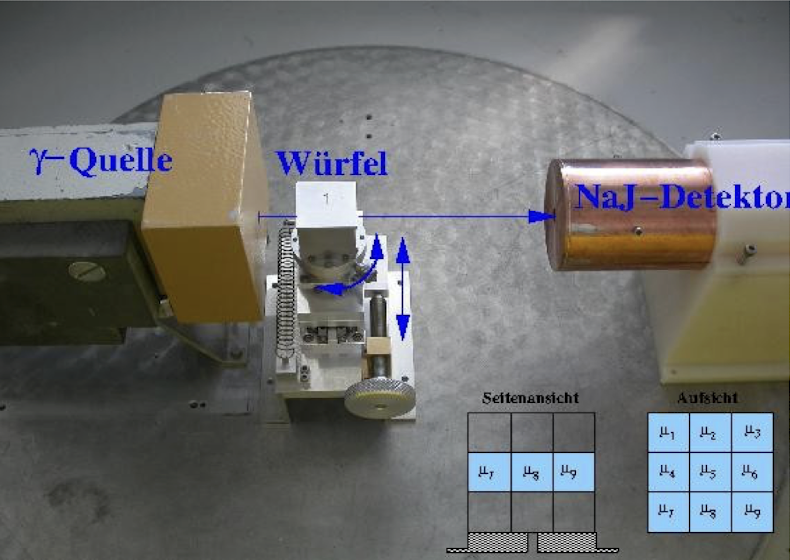
\includegraphics[scale=0.7]{Abbildungen/Aufbau.png}
    \caption{Bild von dem Versuchsaufbau.\cite{V14}}
    \label{fig:Aufbau}
\end{figure}
Die Gammaquelle sendet einen kollimierten Strahl aus, welcher auf einen Würfel trifft. 
Jeder Würfel ist $\qty{3}{\centi\meter} \times \qty{3}{\centi\meter} \times \qty{3}{\centi\meter}$ groß und besteht aus $3 \times 3 \times 3$
Elementarwürfeln, die eime Seitenlänge von $\qty{1}{\centi\meter}$ besitzen. Die Elementarwürfel werden von einer Aluminiumhülle mit einer
Wandstärke von $\qty{1}{\milli\meter}$ umgeben.\\
Es gibt vier unterschiedliche Ausführungen von diesem Würfel. Der erste Würfel besteht nur aus der Aluminiumhülle.
Beim zweiten und dritten Würfel bestehen alle in der Aluminiumhülle enthaltenen Elementarwürfel nur aus einem Material. Der vierte Würfel besteht aus
einer Mischung von Elementarwürfeln verschiedener Materialien.
Die möglichen Materialien aus denen die Elementarwürfel bestehen können sind Aluminium, Messing, Delrin, Blei und Eisen.
Der durchstrahlte Würfel kann um seine z-Achse gedreht werden und senkrecht zur Strahlrichtung verschoben werden.
Der Strahl wird nach dem Durchlaufen des Würfels von einem NaJ-Detektor aufgenommen, wobei das Material im Szintillatordetektor durch die einfallende
Strahlung angeregt wird. Bei Abregung des Materials werden Photonen emittiert, welche auf eine Photokathode treffen. Die dort durch den Photoeffekt
ausgelösten Elektronen werden im Photomultiplier beschleunigt und vermehrt und ein elektrisches Signal wird erzeugt.
Die so erzeugten Pulse werden von einem Vorverstärker verstärkt.
Anschließend werden diese Pulse von einem Multichannelanalyser analysiert, indem das Signal entsprechend seiner Größe einem Kanal innerhalb des Datensatzes zugeordnet wird.
An einem Spektroskopie Amplifier werden die Detektorspannung und die Vorverstärkerspannung eingestellt. Das Einstellen der Diskriminatorschwelle und die Datenaufnahme
werden über den Computer und das Programm MAESTRO durchgeführt.



\section{Durchführung}
\label{sec:Durchführung}
Zuerst wird das Spektrum der Quelle bestimmt, ohne Abschwächung des Strahls, also ohne einen Würfel im Strahlengang.
Dabei sollen alle Prozesse des Spektrums identifiziert werden.
Es wird bei allen Messungen über einem Zeitraum von jeweils $t = \qty{300}{\second}$ gemessen.

Anschließend wird die Messung an jeweils einem der vier Würfel durchgeführt und die Werte aufgenommen.
Es wird nur die mittlere Schicht des Würfels untersucht, aufgrund von Zeitgründen.
Der Würfel 1 wird entlang der $I_2$ Richtung durchstrahlt und die Werte des Photopeaks aufgenommen.
Bei den homogenen Würfeln wird aus vier Richtungen gemessen, der Würfel mit den verschiedenen 
Elementarwürfeln wird aus allen 12 Richtungen durchstrahlt(siehe \autoref{fig:Ausrichtung}).

\section{Vorbereitung}
\label{sec:Vorbereitung}
Zur Bestimmung des Abschwächungskoeffizient wird die Matrix $A$ benötigt, welche die Informationen der Wegstrecke enthält. \autoref{eqn:muMatrix} lässt sich schreiben zu
\begin{equation}
    d \cdot
    \begin{pmatrix}
        1 & 0 & 0 & 1 & 0 & 0 & 1 & 0 & 0 \\
        0 & 1 & 0 & 0 & 1 & 0 & 0 & 1 & 0 \\
        0 & 0 & 1 & 0 & 0 & 1 & 0 & 0 & 1 \\
        1 & 1 & 1 & 0 & 0 & 0 & 0 & 0 & 0 \\
        0 & 0 & 0 & 1 & 1 & 1 & 0 & 0 & 0 \\
        0 & 0 & 0 & 0 & 0 & 0 & 1 & 1 & 1 \\
        0 & \sqrt{2} & 0 & 0 & 0 & \sqrt{2} & 0 & 0 & 0 \\
        \sqrt{2} & 0 & 0 & 0 & \sqrt{2} & 0 & 0 & 0 & \sqrt{2} \\
        0 & 0 & 0 & \sqrt{2} & 0 & 0 & 0 & \sqrt{2} & 0 \\
        0 & 0 & 0 & 0 & 0 & \sqrt{2} & 0 & \sqrt{2} & 0 \\
        0 & 0 & \sqrt{2} & 0 & \sqrt{2} & 0 & \sqrt{2} & 0 & 0 \\
        0 & \sqrt{2} & 0 & \sqrt{2} & 0 & 0 & 0 & 0 & 0 
    \end{pmatrix}
    \cdot
    \begin{pmatrix}
        \mu_1 \\
        \mu_2 \\
        \mu_3 \\
        \mu_4 \\
        \mu_5 \\
        \mu_6 \\
        \mu_7 \\
        \mu_8 \\
        \mu_9 
    \end{pmatrix}
    =
    \begin{pmatrix}
        I_1 \\
        I_2 \\
        I_3 \\
        I_4 \\
        I_5 \\
        I_6 \\
        I_7 \\
        I_8 \\
        I_9 \\
        I_{10} \\
        I_{11} \\
        I_{12} 
    \end{pmatrix}
    .
\end{equation}

In \autoref{tab:abs_literatur} sind die Absorptionskoeffizienten für die möglichen Materialien der Elementarwürfel aufgeslistet.
Durch den Vergleich der errechneten Absorptionskoeffizienten kann so bestimmt werden, aus welchen Materialien die Würfel bestehen.
